%%%%%%%%%%%%%%%%%%%%%%%%%%%%%%%%%%%
%This is the LaTeX ARTICLE template for RSC journals
%Copyright The Royal Society of Chemistry 2016
%%%%%%%%%%%%%%%%%%%%%%%%%%%%%%%%%%%

\documentclass[twoside,twocolumn,9pt]{article}
\usepackage{extsizes}
\usepackage[super,sort&compress,comma]{natbib} 
\usepackage[version=3]{mhchem}
\usepackage[left=1.5cm, right=1.5cm, top=1.785cm, bottom=2.0cm]{geometry}
\usepackage{balance}
\usepackage{mathptmx}
\usepackage{sectsty}
\usepackage{graphicx} 
\usepackage{lastpage}
\usepackage[format=plain,justification=justified,singlelinecheck=false,font={stretch=1.125,small,sf},labelfont=bf,labelsep=space]{caption}
\usepackage{float}
\usepackage{fancyhdr}
\usepackage{fnpos}
\usepackage[english]{babel}
\addto{\captionsenglish}{%
  \renewcommand{\refname}{Notes and references}
}
\usepackage{array}
\usepackage{droidsans}
\usepackage{charter}
\usepackage[T1]{fontenc}
\usepackage[usenames,dvipsnames]{xcolor}
\usepackage{setspace}
\usepackage[compact]{titlesec}
\usepackage{hyperref}
%%%Please don't disable any packages in the preamble, as this may cause the template to display incorrectly.%%%

\usepackage{epstopdf}%This line makes .eps figures into .pdf - please comment out if not required.

\definecolor{cream}{RGB}{222,217,201}
\definecolor{jlblue}{rgb}{0.0,0.6056031611752245,0.9786801175696073}
\definecolor{jlorange}{rgb}{0.8888735002725198,0.43564919034818994,0.2781229361419438}
\definecolor{jlgreen}{rgb}{0.2422242978521988,0.6432750931576305,0.3044486515341153}
\definecolor{jlviolet}{rgb}{0.7644401754934356,0.4441117794687767,0.8242975359232758}

\begin{document}

\pagestyle{fancy}
\thispagestyle{plain}
\fancypagestyle{plain}{
%%%HEADER%%%
\renewcommand{\headrulewidth}{0pt}
}
%%%END OF HEADER%%%

%%%PAGE SETUP - Please do not change any commands within this section%%%
\makeFNbottom
\makeatletter
\renewcommand\LARGE{\@setfontsize\LARGE{15pt}{17}}
\renewcommand\Large{\@setfontsize\Large{12pt}{14}}
\renewcommand\large{\@setfontsize\large{10pt}{12}}
\renewcommand\footnotesize{\@setfontsize\footnotesize{7pt}{10}}
\makeatother

\renewcommand{\thefootnote}{\fnsymbol{footnote}}
\renewcommand\footnoterule{\vspace*{1pt}% 
\color{cream}\hrule width 3.5in height 0.4pt \color{black}\vspace*{5pt}} 
\setcounter{secnumdepth}{5}

\makeatletter 
\renewcommand\@biblabel[1]{#1}            
\renewcommand\@makefntext[1]% 
{\noindent\makebox[0pt][r]{\@thefnmark\,}#1}
\makeatother 
\renewcommand{\figurename}{\small{Fig.}~}
\sectionfont{\sffamily\Large}
\subsectionfont{\normalsize}
\subsubsectionfont{\bf}
\setstretch{1.125} %In particular, please do not alter this line.
\setlength{\skip\footins}{0.8cm}
\setlength{\footnotesep}{0.25cm}
\setlength{\jot}{10pt}
\titlespacing*{\section}{0pt}{4pt}{4pt}
\titlespacing*{\subsection}{0pt}{15pt}{1pt}
%%%END OF PAGE SETUP%%%

%%%FOOTER%%%
\fancyfoot{}
\fancyfoot[LO,RE]{\vspace{-7.1pt}
\includegraphics[height=9pt]{head_foot/LF}}
\fancyfoot[CO]{\vspace{-7.1pt}\hspace{13.2cm}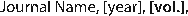
\includegraphics{head_foot/RF}}
\fancyfoot[CE]{\vspace{-7.2pt}\hspace{-14.2cm}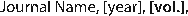
\includegraphics{head_foot/RF}}
\fancyfoot[RO]{\footnotesize{\sffamily{1--\pageref{LastPage} ~\textbar  \hspace{2pt}\thepage}}}
\fancyfoot[LE]{\footnotesize{\sffamily{\thepage~\textbar\hspace{3.45cm} 1--\pageref{LastPage}}}}
\fancyhead{}
\renewcommand{\headrulewidth}{0pt} 
\renewcommand{\footrulewidth}{0pt}
\setlength{\arrayrulewidth}{1pt}
\setlength{\columnsep}{6.5mm}
\setlength\bibsep{1pt}
%%%END OF FOOTER%%%

%%%FIGURE SETUP - please do not change any commands within this section%%%
\makeatletter 
\newlength{\figrulesep} 
\setlength{\figrulesep}{0.5\textfloatsep} 

\newcommand{\topfigrule}{\vspace*{-1pt}% 
\noindent{\color{cream}\rule[-\figrulesep]{\columnwidth}{1.5pt}} }

\newcommand{\botfigrule}{\vspace*{-2pt}% 
\noindent{\color{cream}\rule[\figrulesep]{\columnwidth}{1.5pt}} }

\newcommand{\dblfigrule}{\vspace*{-1pt}% 
\noindent{\color{cream}\rule[-\figrulesep]{\textwidth}{1.5pt}} }

\makeatother
%%%END OF FIGURE SETUP%%%

%%%TITLE, AUTHORS AND ABSTRACT%%%
\twocolumn[
  \begin{@twocolumnfalse}
{
\includegraphics[height=30pt]{head_foot/SM}\hfill\raisebox{0pt}[0pt][0pt]{
\includegraphics[height=55pt]{head_foot/RSC_LOGO_CMYK}}\\[1ex]

\includegraphics[width=18.5cm]{head_foot/header_bar}}\par
\vspace{1em}
\sffamily
\begin{tabular}{m{4.5cm} p{13.5cm} }


\includegraphics{head_foot/DOI} & \noindent\LARGE{\textbf{Instabilities of ring-rivulets: Impact of wettability gradients$^\dag$}} \\%Article title goes here instead of the text "This is the title"
\vspace{0.3cm} & \vspace{0.3cm} \\

 & \noindent\large{Stefan Zitz,\textit{$^{a}$} Andrea Scagliarini,\textit{$^{b,c}$} Johan Roenby\textit{$^{a}$}} \\%Author names go here instead of "Full name", etc.

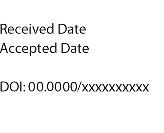
\includegraphics{head_foot/dates} & \noindent\normalsize{
Rivulets and droplets are naturally appearing shapes when small amounts of liquid are brought into contact with a partially wettable substrate.
Here we study, by the means of numerical simulations, the dynamics of a ring-rivulet placed on a solid substrate.
First we consider a uniform substrate, similar to the work of Nguyen \textit{et al. Langmuir}, 2012, \textbf{28}, 13960-13967.
We then consider different kinds of surface patterns and show that they not only affect the stability but also the morphology.
Thus making it possible to enhance the probability for a Rayleigh-Plateau type break up into multiple droplets or to accelerate the capillary retraction that stems from the curvature difference of the ring and leads to a single droplet.
}

\end{tabular}

 \end{@twocolumnfalse} \vspace{0.6cm}

]
%%%END OF TITLE, AUTHORS AND ABSTRACT%%%

%%%FONT SETUP - please do not change any commands within this section
\renewcommand*\rmdefault{bch}\normalfont\upshape
\rmfamily
\section*{}
\vspace{-1cm}


%%%FOOTNOTES%%%

\footnotetext{\textit{$^{a}$~IMFUFA, Department of Science and Environment, Roskilde University, Postbox 260, 4000 Roskilde, DK. Tel: +45 2993 1923; E-mail: johan@ruc.dk}}
\footnotetext{\textit{$^{b}$~Institute for Applied Mathematics "M. Picone" (IAC), Consiglio Nazionale delle Ricerche (CNR), Via dei Taurini 19, 00185 Rome, Italy, E-mail: andrea.scagliarini@cnr.it}}
\footnotetext{\textit{$^{c}$~INFN, sezione Roma ``Tor Vergata'', via della Ricerca Scientifica 1, 00133 Rome, Italy}}


%Please use \dag to cite the ESI in the main text of the article.
%If you article does not have ESI please remove the the \dag symbol from the title and the footnotetext below.
\footnotetext{\dag~Electronic Supplementary Information (ESI) available: \href{https://github.com/Zitzeronion/Ring_rivulets}{Ring\_rivulets}. See DOI: 10.1039/cXsm00000x/}
%additional addresses can be cited as above using the lower-case letters, c, d, e... If all authors are from the same address, no letter is required

%\footnotetext{\ddag~Additional footnotes to the title and authors can be included \textit{e.g.}\ `Present address:' or `These authors contributed equally to this work' as above using the symbols: \ddag, \textsection, and \P. Please place the appropriate symbol next to the author's name and include a \texttt{\textbackslash footnotetext} entry in the the correct place in the list.}


%%%END OF FOOTNOTES%%%

%%%MAIN TEXT%%%%
\section{Introduction}
\label{sec:intro}
Thin films and droplets play in an important role in our everyday life.
They are the basis for a host of natural and technological applications~\cite{degennesCapillarityWettingPhenomena2004, ronsinPhaseFieldSimulationsMorphology2022, fockeLabonaFoilMicrofluidicsThin2010}.
Understanding their dynamics and controlling their stability is a central problem for applied research in process engineering and nanotechnology~\cite{singhInkjetPrintingProcess2010, quereFluidCoatingFiber1999, utadaDrippingJettingDrops2007}, but also poses a fundamental physical problem~\cite{oronLongscaleEvolutionThin1997, beckerComplexDewettingScenarios2003, thielePatternedDepositionMoving2014, wilczekSlidingDropsEnsemble2017, peschkaSignaturesSlipDewetting2019}.
One of the more commonly known example that have been theoretically explored are coatings. 
During the coating process the coverage of the film relies heavily on the wettability of the surface. 
Impurities on the surface or instabilities on the film can actually damage the coating and lead wrinkling, to hole formation or dewetting~\cite{bonnWettingSpreading2009, chenWrinklingInstabilitiesPolymer2012}. 
To simulate this systems one has to overcome and inherent multiscale problem, that spans from the molecular motion at the three phase contact line to the nano-/mircoscale thickness of the film up to the macroscopic area the coating covers. 

A thin film model can also be used to study the dynamics of ring-rivulet on a solid substrate.
This particular fluid structure has been point of interest to previous studies~\cite{nguyenCompetitionCollapseBreakup2012, gonzalezStabilityLiquidRing2013, wuCompetingLiquidPhase2011} and differs considerably from a straight liquid rivulet~\cite{diezBreakupFluidRivulets2009, diezStabilityFinitelengthRivulet2009, diezInstabilityTransverseLiquid2012} due to the introduction of multiple unbalanced curvatures.
Recently, Suo et al.~\cite{suoDewettingCornerFilm2023a} have studied a related problem where the film admits a wedge shape and a solid cylinder fills the inner part of the ring. 
The ring is therefore not allowed to contract, but can breakup and form droplets.
They further show a good agreement between theory and simulations as well as a clear dependence of the dynamics on the initial width of the film and the contact angles at each boundary.
Self- and direct assembly of nanomaterials from liquid nanostructures has been one of the driving forces for the study of Nguyen et al.~\cite{nguyenCompetitionCollapseBreakup2012} and earlier studies of Wu et al.~\cite{wuBreakupPatternedNanoscale2010} where they showed that liquid-metal rings are suited to form arrays of droplets.
Diez et al.~\cite{diezBreakupFluidRivulets2009, diezStabilityFinitelengthRivulet2009} laid the theoretical foundation for a straight rivulet in their work using linear stability analysis (LSA) and numerical simulations. 
Later, Gonz{\'a}lez et al.~\cite{gonzalezStabilityLiquidRing2013} extend these results towards a cut torus shape and called it liquid ring, making it therefore possible to predict wavelengths for the most unstable mode and describing the competing time scales for collapse and breakup.
In their study they however point out that for thin films, where the disjoining pressure~\cite{schwartzSimulationDropletMotion1998, beckerComplexDewettingScenarios2003, oronLongscaleEvolutionThin1997} can not be ignored, e.g. a few nanometres in thickness, the LSA overpredicts  the expected number of droplets after breakup.
While the disjoining pressure model seems to choose a larger wavelength before breakup Nguyen et al.~\cite{nguyenCompetitionCollapseBreakup2012} showed that molecular dynamics (MD) simulations seem to agree with the LSA when it comes to the number of droplets.
Beside the work on thin films Mehrabian and Feng~\cite{mehrabianCapillaryBreakupLiquid2013} showed simulations and experiments of a freely suspend liquid torus in another fluid.
In their study they found that the time to breakup depends inversely on the amplitude of the initial perturbation and the initial thickness of the torus.
They further discuss the influence of the viscosity contrast between the liquids, as this difference has an effect both on the capillary waves and the retraction velocities.

We are going to address the thin ring-rivulet problem with a further complication, namely the introduction of a wettability gradient.
With recent developments in surface chemistry and the emerging technology of switchable substrates~\cite{xinReversiblySwitchableWettability2010, stuartEmergingApplicationsStimuliresponsive2010,chenThermalresponsiveHydrogelSurface2010, ichimuraLightDrivenMotionLiquids2000, mugeleElectrowettingConvenientWay2005} local precise wettability gradients are more attainable than ever.
It has been shown numerous times that wettability gradients are able to transport droplets, see ref.~\cite{liuActuatingWaterDroplets2015} or more recently with time dependent patterns refs.~\cite{grawitterSteeringDropletsSubstrates2021, zitzControllingDewettingMorphologies2023}, thus having a wettability gradient should allow for a more fine grained the control of the intermediate ring-rivulet states.
To this end we show that it is possible to actively control the number of droplets after breakup and furthermore be even able to set the spacing between neighboring droplets.
Having arbitrary control over these quantities will in fact make this process more applicable for the production of nanomaterials. 

The outline of the paper is as follows: In the next section, Sec.~\ref{sec:method} we introduce the method we use to run numerical experiments.
We then present our results in Sec.~\ref{sec:dynamics}, starting with a comparison with the literature and then present the impact of the wettability gradient.
In the last section, Sec.~\ref{sec:conclu} we give a short summary, highlighting important results and conclude with an outlook of possible research applications.

\section{Simulation method}
\label{sec:method}
For the time resolved simulations of a thin liquid ring-rivulet we use a recently developed lattice Boltzmann method (LBM) for thin films~\cite{zitzLatticeBoltzmannMethod2019, zitzLatticeBoltzmannSimulations2021, zitzSwalbeJlLattice2022, zitzControllingDewettingMorphologies2023}. 
Here we quickly introduce the method and highlight the relevant modelling approximations.
The thin film model is build on a class of LBMs originally proposed for shallow water systems~\cite{salmonLatticeBoltzmannMethod1999, dellarNonhydrodynamicModesPriori2002}.
The master equation for the evolution of the discrete probability functions $f_l(\mathbf{x},t)$ of a fluid system subject to a forcing $\mathbf{F}_{\mbox{\tiny{tot}}}$ reads
\begin{equation}\label{eq:LBE}
\begin{split}
&f_l(\mathbf{x}+\mathbf{c}^{(l)}\Delta t,t+\Delta t) = \\
&(1 - \omega) f_l(\mathbf{x},t) + \omega f_l^{(eq)}(\mathbf{x},t) + w_l \frac{\Delta t}{c_s^2} \mathbf{c}^{(l)} \cdot \mathbf{F}_{\mbox{\tiny{tot}}},
\end{split}
\end{equation}
where the discrete lattice velocities $\mathbf{c}_l$ run from $0$ to $8$ in our two-dimensional scheme and $\mathbf{x} = (x,y)$.
This equation admits a local collision step in which the distribution functions are relaxed towards their equilibrium $f_l^{(eq)}(\mathbf{x},t)$ with relaxation rate $\omega = \Delta t/\tau$ and a non-local streaming step, where the $f_l(\mathbf{x},t)$ are streamed to their nearest neighbours.
The relaxation time $\tau$, within this study we set $\tau = 1$, is proportional to the fluid's kinematic viscosity $\nu$, which is set to $\nu = 1/6$.  
The remaining parameters, namely $c_s$, $\mathbf{c}^{(l)}$ and $w_l$, are the speed of sound, discrete lattice velocities and the lattice weights. 
We use the standard $D2Q9$ (athermal) values, therefore $c_s = 1/\sqrt{3}$, the lattice velocities are set using~\cite{krugerLatticeBoltzmannMethod2017, zitzLatticeBoltzmannMethod2019, salmonLatticeBoltzmannMethod1999}   
\begin{equation}\label{eq:speeds}
\mathbf{c}^{(l)}  =
\left\{
\begin{array}{ll}
(0,0) & l = 0 \\
\left[\cos{\frac{(l-1)\pi}{4}}, \sin{\frac{(l-1)\pi}{4}} \right] &  l=1,3,5,7 \\
\sqrt{2}\left[\cos{\frac{(l-1)\pi}{4}}, \sin{\frac{(l-1)\pi}{4}} \right] & l=2,4,6,8
\end{array}
\right.,
\end{equation}
and the weights
\begin{equation}\label{eq:weights}
    w_l  =
    \left\{
    \begin{array}{ll}
        \frac{4}{9} & l = 0 \\
        \frac{1}{9} &  l=1,3,5,7 \\
        \frac{1}{36} & l=2,4,6,8
    \end{array}
    \right..
\end{equation}
The equilibria can be derived using mass, momentum and energy conservation and the set we are using is given by~\cite{salmonLatticeBoltzmannMethod1999, dellarNonhydrodynamicModesPriori2002}  
\begin{equation} \label{eq:equilibria}
f_l^{(eq)}  =
\left\{
\begin{array}{ll}
h - \frac{5gh^2}{6c_s^2} - \frac{2hu^2}{3c_s^2}& l = 0 \\
\frac{gh^2}{6c_s^2} + \frac{h \mathbf{c}^{(l)}\cdot \mathbf{u}}{3 c_s^2} + \frac{h(\mathbf{c}^{(l)}\cdot \mathbf{u})^2}{2 c_s^4}-\frac{hu^2}{6c_s^2} &  l=1,3,5,7 \\
\frac{gh^2}{24c_s^2} + \frac{h \mathbf{c}^{(l)}\cdot\mathbf{u}}{12 c_s^2} + \frac{h (\mathbf{c}^{(l)}\cdot\mathbf{u})^2}{8c_s^4}-\frac{hu^2}{24c_s^2} & l=2,4,6,8
\end{array}
\right.,
\end{equation}
where $u^2 = |\mathbf{u}|^2$ is the magnitude of the velocity.
Upon applying the multiscale Chapman-Enskog expansion~\cite{enskogKinetischeTheorieVorgange1917, chapmanMathematicalTheoryNonuniform1990, krugerLatticeBoltzmannMethod2017} to this LBE and within well defined limits, e.g. $Ma/Fr \ll 1$, where $Fr$ and $Ma$ are the Froude and Mach number respectively, we recover the shallow water system~\cite{salmonLatticeBoltzmannMethod1999, zitzLatticeBoltzmannMethod2019}.

In Eq.~(\ref{eq:LBE}) we left $\mathbf{F}_{\mbox{\tiny{tot}}}$ to be arbitrary, however as discussed in Ref.~\cite{zitzLatticeBoltzmannMethod2019} we can use this term to match the shallow water system to the thin film equation~\cite{oronLongscaleEvolutionThin1997, crasterDynamicsStabilityThin2009, bonnWettingSpreading2009}.
The resulting system of equations reads,
\begin{align}\label{eq:hydro3}
    &\partial_t h + \nabla \cdot (h \mathbf{u})  = 0 \nonumber\\ 
    &\partial_t (h \mathbf{u}) = -gh \nabla h -\frac{1}{\rho_0}h\nabla p_{\mbox{\tiny{film}}} - \nu \alpha_{\delta}(h) \mathbf{u} + \mathbf{F},
\end{align}
where $g$ is the gravitational acceleration, $p_{\mbox{\tiny{film}}}$ is the film pressure
\begin{equation}\label{eq:filmpressure}
    p_{\mbox{\tiny{film}}} = - \gamma\nabla^2 h -\Pi(h),
\end{equation}
with a disjoining pressure~\cite{schwartzSimulationDropletMotion1998,nguyenCompetitionCollapseBreakup2012, gonzalezStabilityLiquidRing2013, zitzControllingDewettingMorphologies2023}
\begin{equation}\label{eq:disjoinpressure}
\Pi(h,\theta) = \frac{2\gamma}{h_{\ast}}[1-\cos\theta(\mathbf{x})]\left[\left(\frac{h_*}{h}\right)^3 -\left(\frac{h_*}{h}\right)^2\right],
\end{equation}
where $\gamma$ is the surface tension which is set to $\gamma = 10^{-2}$ in all numerical experiments.
The space dependent equilibrium contact angle $\theta(\mathbf{x})$, which allows us to ``pattern'' the substrate is set within the bounds $[\pi/18, 2\pi/9]$, with the exception of the banded pattern. 
Lastly $\alpha_{\delta}(h)$ is a substrate friction term that mimics a slip boundary condition with an effective slip length $\delta$
\begin{equation}\label{eq:alphafric}
\alpha_{\delta}(h) = \frac{6h}{(2 h^2 + 6 \delta h + 3 \delta^2)}.
\end{equation}
By introducing a precursor layer $h_{\ast}$ and a slip length $\delta$ we regularize the contact line divergence~\cite{huhHydrodynamicModelSteady1971}. 
The slip length lies within the weak/intermediate slip regime~\cite{peschkaSignaturesSlipDewetting2019,fetzerQuantifyingHydrodynamicSlip2007, munchLubricationModelsSmall2005} and the thickness of the precursor film is set to $h_{\ast} = 0.05$.
Inserting Eqs.~(\ref{eq:filmpressure}\ref{eq:alphafric}) into the second line of Eq.~(\ref{eq:hydro3}) and assuming the quasi-steady limit ($\partial_t(h\mathbf{u}) \approx 0$) we can solve for $\mathbf{u}$.
By applying this solution for $\mathbf{u}$ to the continuity equation we have
\begin{equation}\label{eq:thinsolve}
     \partial_t h(\mathbf{x},t) = \nabla\cdot\left(M_{\delta}(h)\nabla p_{\mbox{\tiny{film}}}\right),
\end{equation}
with the mobility function $M_{\delta}(h) = \frac{h^2}{\mu\alpha_{\delta}(h)}$ which for the no-slip boundary condition $(\delta \rightarrow 0)$ reduces to $M_{0}(h) = h^3/3\mu$.
Without loss of generality we set $\rho_0 = 1$ and thus the dynamic viscosity is $\mu = \rho_0 \nu = 1/6$. 

Our strategy is therefore to iterate Eq.~(\ref{eq:LBE}) in time and find an approximate solution to Eq.~(\ref{eq:thinsolve})~\cite{zitzSwalbeJlLattice2022}.
The numerical domain consists of a square lattice with $512\Delta x$ in both horizontal directions.
We further use biperiodic boundary conditions at the edges of the domain. 

\subsection{Initial conditions}
\begin{figure}
\centering
  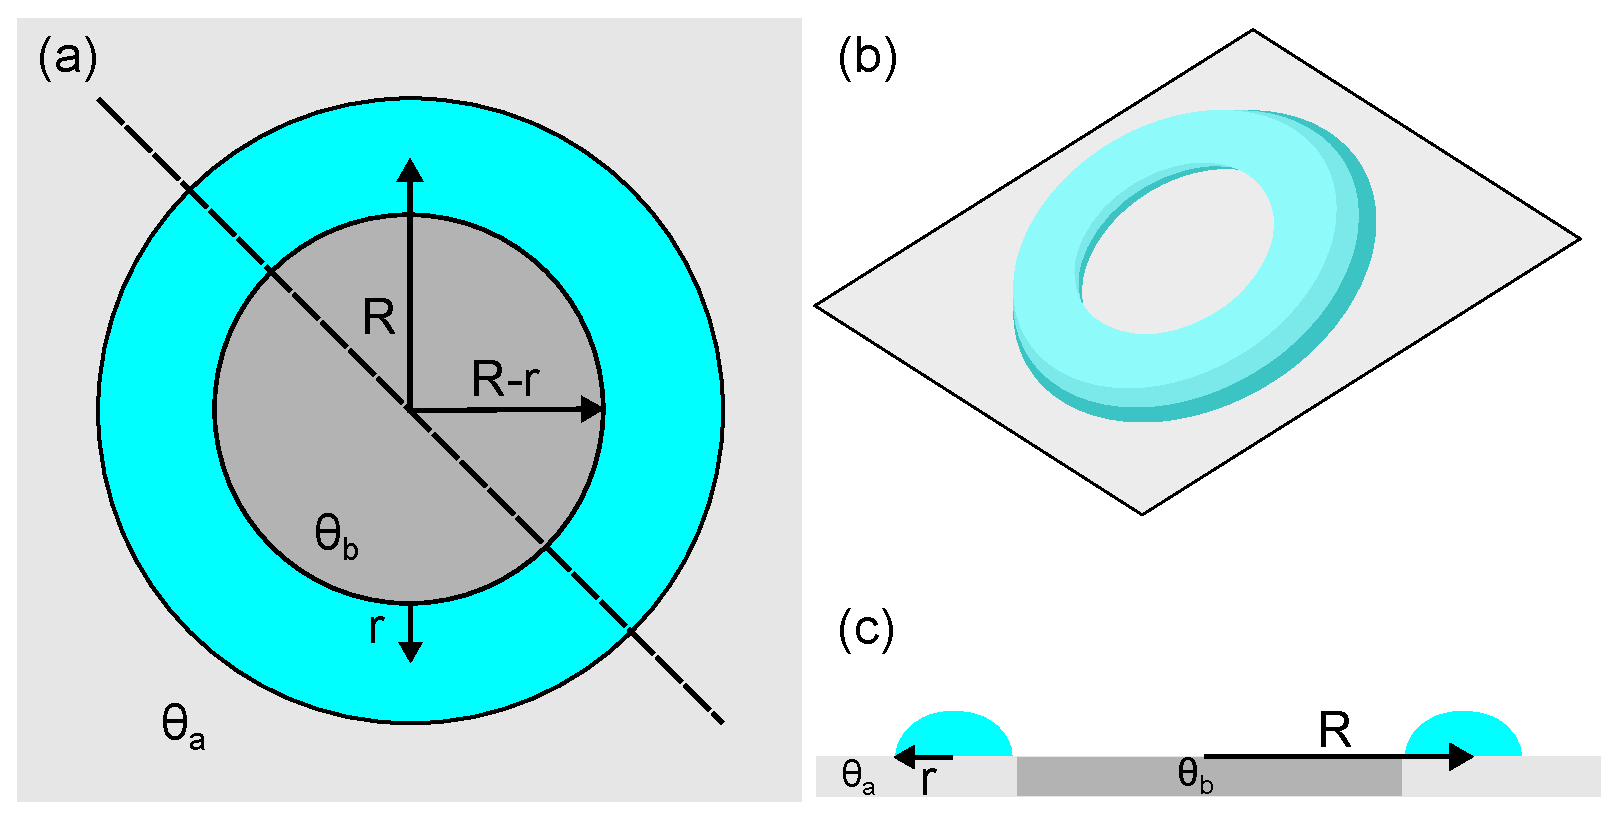
\includegraphics[width=0.45\textwidth]{ringrivulet_shema}
  \caption{Schematic setup of our initial conditions. In (a) we show the top view where $R$ and $r$ are the two different radii and $\theta_a$ and $\theta_b$ can be different contact angles. 
  In (b) we show an isometric view of the initial condition.
  By cutting along the dashed line in (a) we get the side view of (c).}
  \label{fig:ringschema}
\end{figure}

The initial thickness profile $h(\mathbf{x}, t=0)$ of the film is set by an implicit equation for a torus with radial symmetry along the z-axis according to
\begin{equation}\label{eq:torus}
    h(\mathbf{x}, t=0) = \sqrt{r_0^2 - \left(R_0-\xi\right)^2} - r_0\cos(\theta) + \varepsilon(\mathbf{x})\mathcal{N},
\end{equation}
where $\xi = \sqrt{(x-x_0)^2+(y-y_0)^2}$ is a radial coordinate, $R_0$ is the major radius and $r_0$ is the minor radius of the torus.
The center of the torus is at $(x_0,y_0)$ and for all numerical experiments set to the center of the numerical domain $(256,256)$.
Eq.~(\ref{eq:torus}) allows for negative thickness values, however we only consider the upper half of the torus as shown in Fig.~\ref{fig:ringschema}. 
The second term in Eq.~(\ref{eq:torus}) is to cut the upper half to a smaller contact angle.
The third term adds white noise to initial condition, $\mathcal{N}$ is a gaussian with zero mean and $\varepsilon(\mathbf{x})$ is an amplitude that is 
\begin{equation}
    \varepsilon(\mathbf{x}) =
    \begin{cases}
        10^{-2}\quad \textbf{if}~h(\mathbf{x}) > h_{\ast}\\
        0~~\quad\quad \textbf{else}
    \end{cases}
    .
\end{equation} 
We further require that any $h(\mathbf{x}) < 0$ is set to $h_{\ast}$.
The lubrication approximation does in fact not allow us to use the initial conditions in refs.~\cite{nguyenCompetitionCollapseBreakup2012, wuBreakupPatternedNanoscale2010} but are in agreement with Gonz{\'a}lez et al.~\cite{gonzalezStabilityLiquidRing2013}.

Our main interest is focused on the impact of a pattern on the evolution of the ring-rivulet, Eq.~(\ref{eq:torus}). 
As indicated in Fig.~\ref{fig:ringschema} we use different patterns.
A natural starting point that allows to compare to Refs.~\cite{gonzalezStabilityLiquidRing2013, nguyenCompetitionCollapseBreakup2012, wuBreakupPatternedNanoscale2010} is
\begin{equation}\label{eq:theta_const}
    \theta(\xi) = \theta_0,
\end{equation}
where $\theta_0$ is a constant.
In the second scenario we consider a banded case, where the ring-rivulet has the same contact angle as its immediate surrounding and the rest of the substrate has a higher contact angle
\begin{equation}\label{eq:theta_band}
    \theta(\xi) =\begin{cases}
        \theta_a,\quad \text{if}~h(\xi\pm \delta\xi) > 0\\
        \theta_b,\quad \text{else}
    \end{cases}.
\end{equation}
The addition of $\delta\xi$ widens the band and allow the ring-rivulet to contract a bit.  
Lastly, we consider a linear radial wettability gradient towards the middle
\begin{equation}\label{eq:theta_grad}
    \theta(\xi) = \frac{\theta_{a}-\theta_{b}}{R} \xi + \theta_{b},
\end{equation}
where $\theta_{a}\neq\theta_{b}$.
We consider both possibilities, thus a negative wettability gradient ($\theta_a > \theta_b$) and a positive wettability gradient ($\theta_a < \theta_b$).

These three expressions for $\theta$, Eqs.~(\ref{eq:theta_const}-\ref{eq:theta_grad}), are then used in Eq.~(\ref{eq:disjoinpressure}) which is part of the pressure calculation in Eq.~(\ref{eq:thinsolve}).
The numerical experiments therefore create a dynamic response of the initial condition Eq.~(\ref{eq:torus}) to each pattern.

\section{Dynamics of a ring-rivulet}
\label{sec:dynamics}
\begin{figure*}
    \centering
    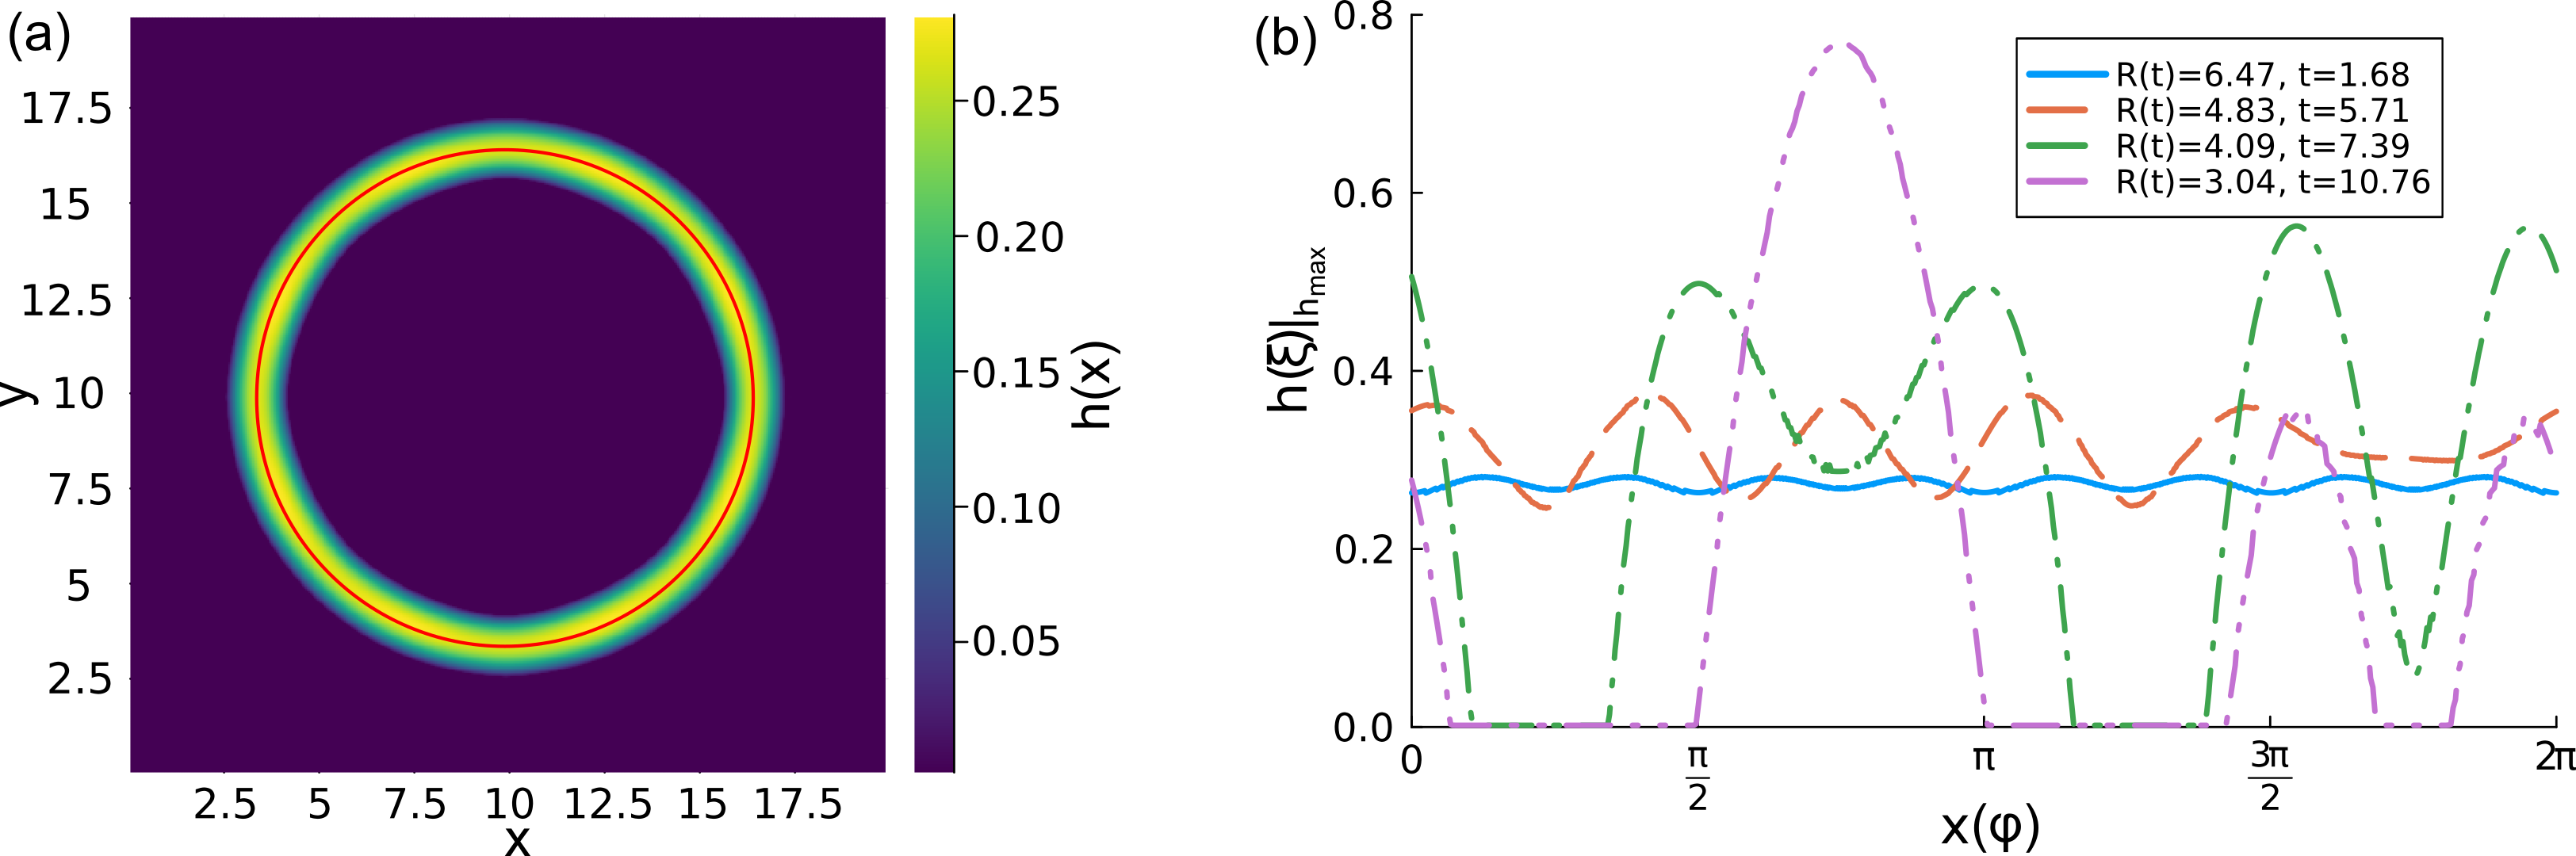
\includegraphics[width=0.95\textwidth]{assets/heatcirc.png}
    \caption{(a) Heatmap of the film thickness at $t=1.68\tau_m$ for $\psi_0 = 0.21$. 
    All length scales are normalized by $H_D = 25.67$. 
    The red ring in the middle of the rivulet is depict as blue line plot in (b).
    In (b) we show circular cuts normalized to $2\pi$, shown in different colors and line styles, for different time steps normalized by Eq.~(\ref{eq:tau_m}) at $\xi(h_{\max})$.
    The ring-rivulet initially chooses a breakup mode that lead to eight droplets, however with time it breaks into three distinct droplets, indicated by the three maxima of the purple curve.}
    \label{fig:ThreeDToOneD}
\end{figure*}
The time resolved dynamics of initial fluid structures Eq.~(\ref{eq:torus}) are surprisingly rich, with one case outlined in Fig.~\ref{fig:ThreeDToOneD}.
It has been shown that the torus geometry is an unstable fluid state~\cite{gonzalezStabilityLiquidRing2013, mehrabianCapillaryBreakupLiquid2013} which is prone to Rayleigh-Plateau and other contact line instabilities. 
The fluid interface itself admits three distinct curvatures, two horizontal ones at the two triple lines between substrate fluid and gas, $\kappa_a = 1/(R+r)$ and $\kappa_b = 1/(R-r)$ as indicated in Fig.~\ref{fig:ringschema}, and one vertical along the liquid-gas interface $\kappa_r = 1/r$.
We remark that both $R$ and $r$ are time dependent quantities that change as the rivulet retracts.
At $t=0$ we have $R_0 = R$ and $r = r_0\sin(\theta)$, thus $r_0$ is the radius of the circle from which the rivulet is cut and at $\theta = \pi/2$ we have $r=r_0$.
These curvatures lead to capillary forces and small instabilities can quickly be amplified and destabilize a torus~\cite{mehrabianCapillaryBreakupLiquid2013} or a liquid ring~\cite{gonzalezStabilityLiquidRing2013}. 
The result can either be a single droplet due to contraction, which is also referred to as collapse or multiple small droplets due to breakup.
Within our numerical experiments we indeed observe both scenarios.

\subsection{Stability and time scales}\label{subsec:stability}
One of the dynamical properties that we are interested in is the stability of the ring-rivulet and the associated time scales.
In previous studies~\cite{gonzalezStabilityLiquidRing2013} the focus was set on the three-phase contact lines and the LSA predictions agreed well with the slip model simulations.
Among the many results of this work is the fact that the varicos modes are always growing stronger than the zigzag modes.
The stability, then, is associated with the width of the ring-rivulet $w = 2r$ as well as the ratio of radii $\psi_0 = 2r/R_0 = w/R_0$.
When the width approaches zero, $w \rightarrow 0$, the rivulet breaks up and is likely to form independent droplets.

We use a slightly different measure to access the stability of the rivulet. 
Instead of directly working with the three-dimensional data we take a circular cut (red circle in Fig.~\ref{fig:ThreeDToOneD}(a)) along the rivuletand measure
\begin{equation}\label{eq:delta-h-measure}
    \Delta h = (h_{\max} - h_{\min})_{\xi = \xi(h_{\max})},
\end{equation}
which can be computed from Fig.~\ref{fig:ThreeDToOneD}(b).
This measure has the advantage that it is well within the rivulet and thus should filter out a constant background from the precursor film $h_{\ast}$.

\begin{figure}
    \centering
    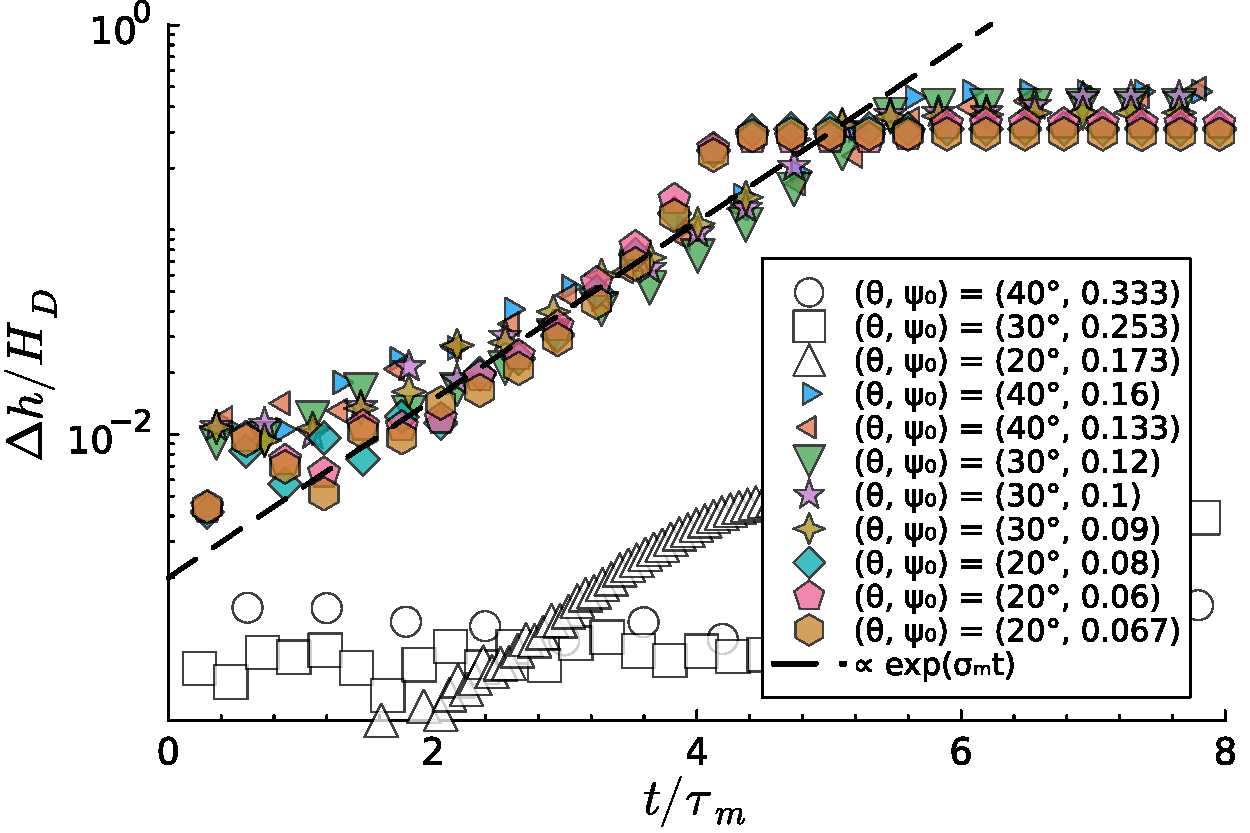
\includegraphics[width=0.45\textwidth]{assets/growth-breakup.pdf}
    \caption{Thickness difference $\Delta h$ normalized by the height of a spherical cap droplet that contains all liquid $H_D$ along the curve at radius $\xi(h_{\max})$ over time normalized by $\tau_{m}$~\cite{wuBreakupPatternedNanoscale2010} for the uniform pattern, Eq.~(\ref{eq:theta_const}). 
    Different symbols depict different initial conditions. 
    Full or empty symbols distinguish between breakup and collapse. 
    The black dashed curve shows an exponential growth $e^{\sigma_m t}$, see Eq.~(\ref{eq:growth-sigma}).
    }
    \label{fig:first_growth}
\end{figure}
As a criteria for a break up using a circular cut we assume $\Delta h \approx 2\max{h(\mathbf{x},0)}$. 
We know from the LSA that $\Delta h$ should grow exponentially~\cite{wuBreakupPatternedNanoscale2010, gonzalezStabilityLiquidRing2013, nguyenCompetitionCollapseBreakup2012}.
To address this statement we use the growth rate $\sigma_m$ which reads
\begin{equation}\label{eq:growth-sigma}
    \sigma_m = \frac{\gamma a \theta^{3/2}\sqrt{\theta - \sin(2\theta)/2}}{6\mu\sin(\theta)\sqrt{A}}, 
\end{equation}
where $a$ is a numerical constant which is set to $a = 0.0379$ according to Ref.~\cite{wuBreakupPatternedNanoscale2010, diezBreakupFluidRivulets2009} and $A$ is half of the area of the cross-section of the rivulet as shown in Fig.~\ref{fig:ringschema}(c).
We like to mention that Eq.~(\ref{eq:growth-sigma}) differs from ref~\cite{wuBreakupPatternedNanoscale2010} by a factor of $\theta^{-3/2}$, however using $\sigma_m$ we can derive a timescale $\tau_m$ by simply inverting the growth rate  
\begin{equation}\label{eq:tau_m}
    \tau_{m} = \frac{1}{\sigma_m} = \frac{6\mu\sin(\theta)\sqrt{A}}{\gamma a \theta^{3/2}\sqrt{\theta - \sin(2\theta)/2}}.      
\end{equation}
In Fig.~\ref{fig:first_growth} we show $\Delta h$ data at different time steps for the uniform pattern normalized by their respective $H_D$ and $\tau_m$ as the different symbols.  
We find a reasonable collapse for the full symbols with this rescaling and as a guide to eye we add a black dashed line that is proportional to $e^{\sigma_m t}$, see Eq.~(\ref{eq:growth-sigma}). 
The empty symbols on the other hand do not show a pronounced growth, with the one exception of the open triangles ($\triangle$, $\psi_0 = 0.173$). 
The filled symbols are numerical experiments that lead to break up of the rivulet, while the empty symbols display the collapse into a single droplet.

Therefore, the $\Delta h$ values along $\xi(h_{\max})$ of the rivulet allow us to distinguish between initial conditions that lead to breakups and droplet fragmentation, as such following the dashed line in Fig.~\ref{fig:first_growth}, and a collapse into a single droplet as shown by the open symbols in Fig.~\ref{fig:first_growth}.
The open triangles ($\triangle$, $\psi_0 = 0.173$) actually mark an edge case in which $\Delta h$ grows with a similar slope as the filled symbols, however the timescale on which the instability grows is too long as compared to the collapse timescale. 
We will get back to this point in Sec.~\ref{subsec:wettability} where we discuss the banded case, Eq.~(\ref{eq:theta_band}) and show that the collapse is fast for larger $\psi_0$s as compared to the breakup instability.

\subsection{Droplets and time scales}\label{subsec:drop-counting}
\begin{figure}
    \centering
    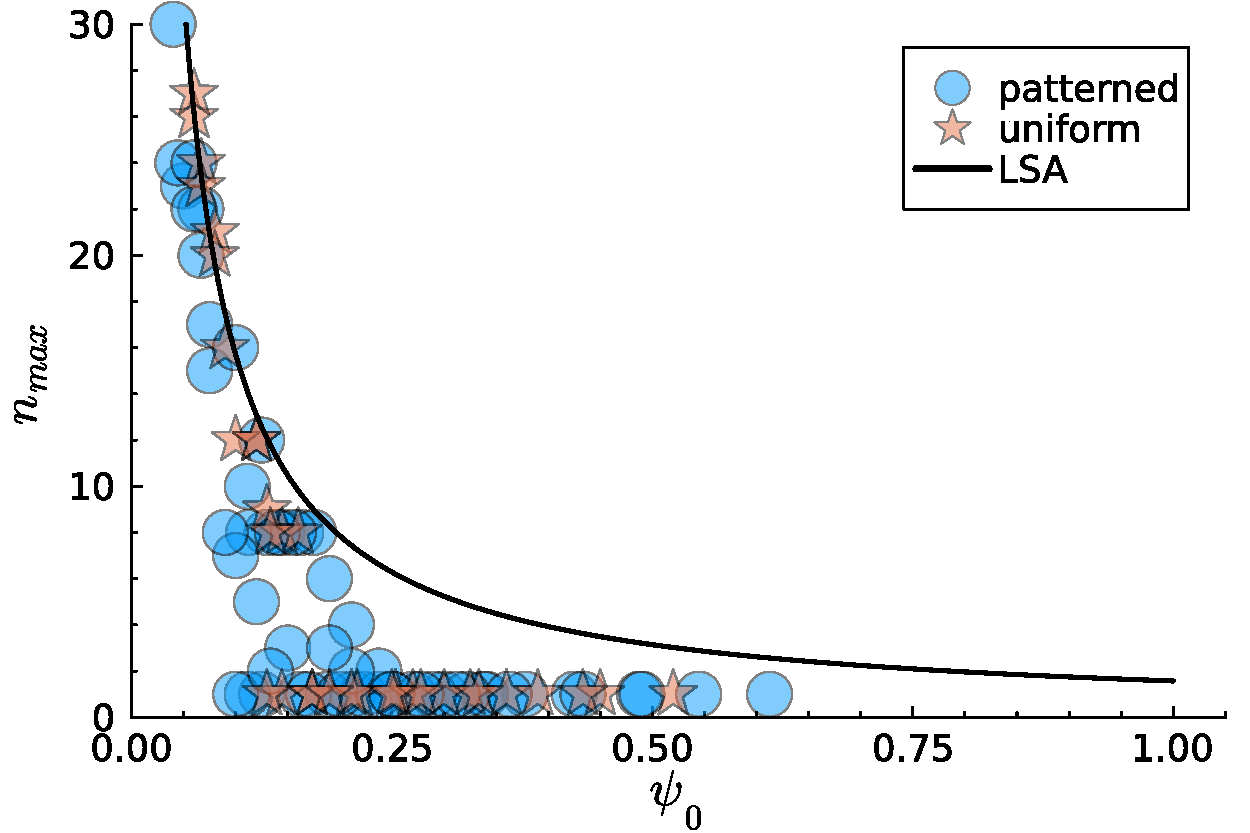
\includegraphics[width=0.45\textwidth]{assets/LSA_droplets.pdf}
    \caption{Number of maximal droplets $n_{max}$ over reduced aspect ratio $\psi_0$.
    Different symbols show different substrates, where Eq.~(\ref{eq:theta_const}) is shown by blue bullets (\textcolor{jlblue}{$\bullet$}) and Eq.~(\ref{eq:theta_band}) by orange stars (\textcolor{jlorange}{$\star$}).
    We compare our results to the linear stability analysis (LSA) from Gonz{\'a}lez et al.~\cite{gonzalezStabilityLiquidRing2013}}
    \label{fig:max_drops}
\end{figure}

Given the initial conditions of the ring-rivulet can we predict if there is a collapse or a brake up and if the rivulet breaks during contraction how many droplets are formed?
While this may sound like a funny question it bares great impact for nanostructuring and/or self-assembly, thus having predictive power is of great interest.
Both questions were addressed by Gonz{\'a}lez et al.~\cite{gonzalezStabilityLiquidRing2013}. 
The maximal number of droplets $n_{\max}$ can be computed with a complex system of equations which are based on the most unstable mode.
They furthermore found a surprisingly good approximation that can be calculated from initial conditions, 
\begin{equation}\label{eq:maxDrops}
    n_{\max, app} = \frac{\pi}{2\psi_0}.
\end{equation}
Therefore, it seems as if the number of droplets is simply set at $t=0$.
This result has been tested and shown to agree well with MD simulations by Nguyen et al.~\cite{nguyenCompetitionCollapseBreakup2012}. 

However, Gonz{\'a}lez et al.~\cite{gonzalezStabilityLiquidRing2013} pointed out as well that the LSA and thus $n_{\max}$ fall short if one considers a disjoining pressure model, see e.g., Eq.~(\ref{eq:disjoinpressure}).
They report that although initially the rivulet adapts to its most unstable mode it does not necessary break up into $n_{\max}$ droplets, especially for $\psi_0 > 0.15$. 
They also point towards the experiments of Wu et al.~\cite{wuCompetingLiquidPhase2011} where a similar mismatch with theoretical predictions was observed.

We perform a similar analysis and count the number of droplets during our numerical experiments and adopted the scheme introduced by Gonz{\'a}lez et al.~\cite{gonzalezStabilityLiquidRing2013}, thus count the collapse as zero droplets, one off center droplet as one, two droplets as two and so on.
The result is shown in Fig.~\ref{fig:max_drops}, where the black line is given by Eq.~(\ref{eq:maxDrops}) and the different symbols refer to different patterns, see Eqs.(~\ref{eq:theta_const}-\ref{eq:theta_band}).
Our results agree with the observations made by Gonz{\'a}lez et al.~\cite{gonzalezStabilityLiquidRing2013} and in Fig.~\ref{fig:ThreeDToOneD} we actually observe a transition from $n = 8$ (blue curve) to $n = 3$ (purple curve).

% We can further quantify this behavior in terms of time scales for both the collapse and the breakup of the ring-rivulet.
In Fig.~\ref{fig:max_drops} we see that for larger $\psi_0$-values theory and our numerical experiments do not agree.
In fact, for $\psi_0 > 0.22$ the ring-rivulet on the homogeneous substrate favors the collapse $n = 0$, with a few outliers. 
It is therefore fair to assumes that the growth-rate of the instability is slower than the the rate of collapse, thus $t_b > t_c$ for $\psi_0 > 0.22$, see Fig.~\ref{fig:first_growth} empty symbols.
In Fig.~\ref{fig:timescaleDifference} we measured these time scales as function of $\psi_0$ and normalized them with their respective $\tau_m$ Eq.~(\ref{eq:tau_m}).
\begin{figure}
    \centering
    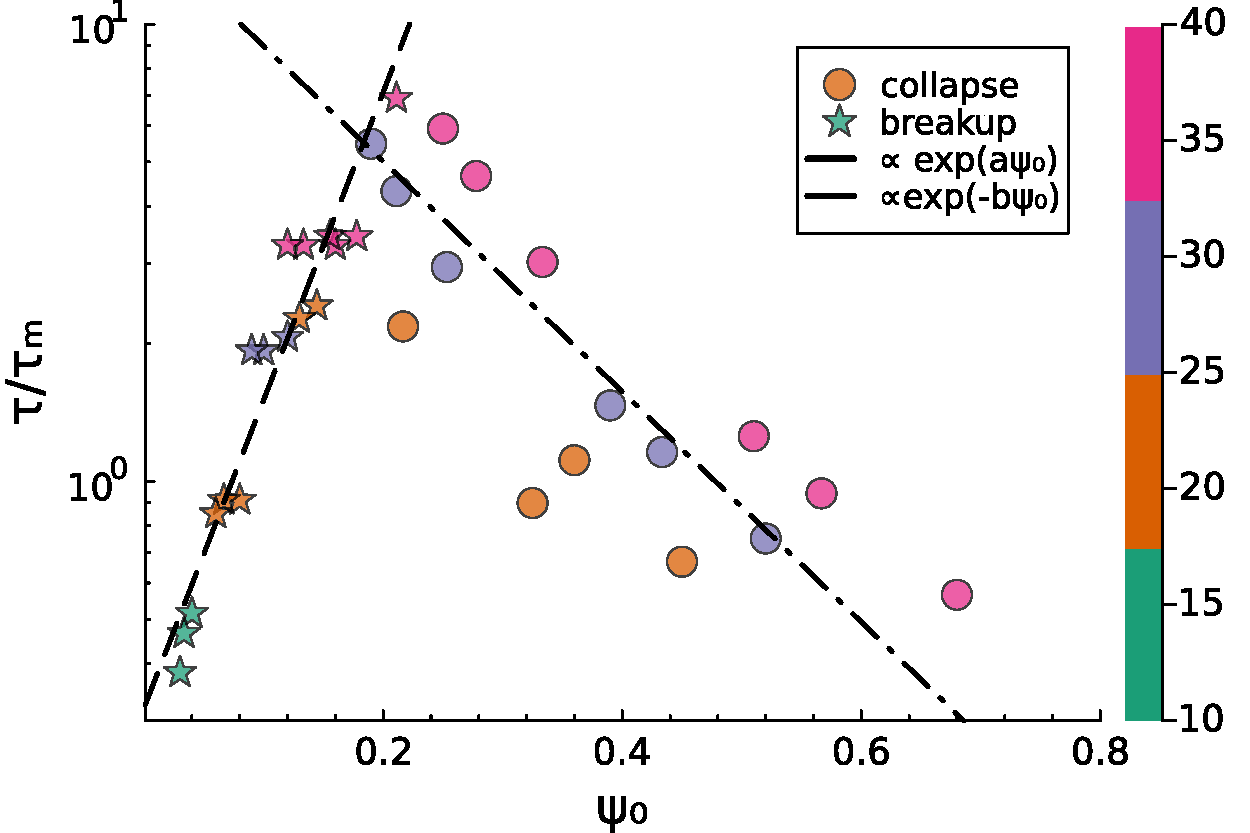
\includegraphics[width = 0.45\textwidth]{assets/uniform_timescales.pdf}
    \caption{Breakup and collapse times $\tau$ for all numerical experiments on a uniform substrate, Eq.~(\ref{eq:theta_const}).
        On the x-axis we use the dimensionless length scale $\psi_0$ and the y-axis displays either the breakup- or collapse time $\tau$ with stars (\textcolor{jlorange}{$\star$}) or bullets (\textcolor{jlblue}{$\bullet$}) respectively.
        The dashed line serves as a guide to eye and shows an exponential growth that is in agreement with the breakup data. 
        The dash-dotted line shows and exponential decay which can be motivated by the collapse data.
        % We do not observe breakup events for ring-rivulets with $\psi_0 > 0.22$. 
        }
    \label{fig:timescaleDifference}
\end{figure}
First, the data suggest that there is no clear boundary that distinguishes between collapse and breakup.
We find a region around $\psi_0 \approx 0.2$ where the collapse times and the breakup times are of similar magnitude.
On the left side of $\psi_0 \approx 0.2$ rivulets are more likely to break up into multiple droplet, while on the right side the collapse is the more likely outcome of a numerical experiment.


\subsection{Wettability patterns}\label{subsec:wettability}


\section{Conclusions}\label{sec:conclu}
We have presented numerical experiments of a liquid ring-rivulet on a uniform and patterned substrate. 
The basis of our experiments is the thin film equation with an additional disjoining pressure model.
First we have confirmed that for small $\psi_0$ values the LSA of Gonz{\'a}lez et al.~\cite{gonzalezStabilityLiquidRing2013} and the measured amount of droplets show good agreement.
For larger values $\psi_0 > 0.1$ the capillary retraction outpaces the breakup and we observe a collapse towards a single droplet or in case of $\theta(x,y)$ is given by Eq.~(\ref{eq:theta_band}) a stable rivulet.



\section*{Author Contributions}
We strongly encourage authors to include author contributions and recommend using \href{https://casrai.org/credit/}{CRediT} for standardised contribution descriptions. Please refer to our general \href{https://www.rsc.org/journals-books-databases/journal-authors-reviewers/author-responsibilities/}{author guidelines} for more information about authorship.

For footnotes in the main text of the article please number the footnotes to avoid duplicate symbols. \textit{e.g.}\ \texttt{\textbackslash footnote[num]\{your text\}}. The corresponding author $\ast$ counts as footnote 1, ESI as footnote 2, \textit{e.g.}\ if there is no ESI, please start at [num]=[2], if ESI is cited in the title please start at [num]=[3] \textit{etc.} Please also cite the ESI within the main body of the text using \dag. For the reference section, the style file \texttt{rsc.bst} can be used to generate the correct reference style.

\section*{Conflicts of interest}
There are no conflicts to declare.

\section*{Acknowledgements}
S. Z. and J. R. acknowledge the financial support from the Independent Research Fund Denmark through a DFF Sapere Aude Research Leader grant (grant number 9063-00018B).



%%%END OF MAIN TEXT%%%

%The \balance command can be used to balance the columns on the final page if desired. It should be placed anywhere within the first column of the last page.

\balance

%If notes are included in your references you can change the title from 'References' to 'Notes and references' using the following command:
%\renewcommand\refname{Notes and references}

%%%REFERENCES%%%
\bibliography{rsc} %You need to replace "rsc" on this line with the name of your .bib file
\bibliographystyle{rsc} %the RSC's .bst file

\end{document}
